\documentclass{beamer}
%\usepackage[scaled]{helvet}
\usepackage[absolute,overlay]{textpos}
\usepackage{amsmath}
\usepackage{graphicx}
\usepackage{tikz}
\usetikzlibrary{shadows}
\usetikzlibrary{shadows.blur}
\usetikzlibrary{patterns}
%\usepackage{kotex}
\usetheme{metropolis}           % Use metropolis theme

% https://github.com/matze/mtheme/issues/308
\usefonttheme{professionalfonts}
\usepackage{unicode-math}
\setmainfont{Fira Sans Light}  % Needs to be specified again!
\setmathfont{TeX Gyre Pagella Math}[Scale=MatchLowercase]  % Just a default
\setmathfont{Fira Sans Light}[range={up/{num,latin,Latin,greek,Greek},%
  \mathexclam,\mathplus,\pm,\div,\minus,\mathpercent,\mathampersand,%
  \mathquestion,\mathatsign,\increment,\less,\equal,\greater,\ne,\leq,%
  \geq,\matheth,\ell,\partial},%
  Script=Latin,script-features={}, sscript-features={}]
\setmathfont{Fira Sans Light Italic}[range={it/{latin,Latin,greek,Greek}},%
  Script=Latin, script-features={}, sscript-features={}]

\title{stateless block verification}
\subtitle{Ethereum Sharding Research}
\date{July 9, 2018}
\author{Jeongho Jeon <maczniak@gmail.com>}
\institute{\textbf{Whitepaper} Foundation, Nonce\\%
(for internal discussion purposes only)}
%\institute{{\fontfamily{phv}\selectfont \textbf{Whitepaper}\\Foundation}, Nonce
%(for internal discussion purposes only)}
\definecolor{boxbg}{HTML}{b4d4eb}
\definecolor{boxredish}{HTML}{ebb4d4}
\definecolor{boxlime}{HTML}{d4ebb4}
\usebackgroundtemplate%
{%
\begin{picture}(50,50)
\put(150,-232){\hbox{\includegraphics[scale=0.1]{whitepaper_colored.png}}}
\end{picture}
%    \includegraphics[width=\paperwidth,height=\paperheight]{whitepaper_colored.png}%
}

\begin{document}

\maketitle

\begin{frame}{Outline}
  \tableofcontents
\end{frame}

\section{Stateless Client Proposal}
\begin{frame}{Stateless Client}
  Vitalik proposed the stateless client idea in Oct 2017.%
  \footnote{https://ethresear.ch/t/the-stateless-client-concept/172}
  It had been discussed until Feb 2018.

  Stateless clients store only headers like Bitcoin SPV, but should verify
  transactions by its own. For stateless clients, the transaction senders (or miners)
  bundle a witness with a transaction. The witness contains state Merkle trees
  of affected accounts.
\end{frame}

\begin{frame}{Advantages}
  \begin{itemize}
    \item Full nodes in general no longer need to store any states.
    \item Fast sync can be done within a few seconds.
    \item Discussions about rent and storage cost disappear.
    \item Disk I/O that was the primary target of DoS attacks decreases.
    \item It supersedes the by-account parallelization (\href{https://github.com/ethereum/EIPs/issues/648}{EIP-648}, that includes affected accounts in a transaction).
    \item State-storing clients can prefetch account storage data from a disk in parallel.
    \item Fast reshuffling nodes across shards helps better security.
  \end{itemize}
\end{frame}

\begin{frame}
  \begin{quote}
    One of Ethereum's key advantages is the platform's ease of use, and the fact that users do not have to care about details like storing private state.
  \end{quote}
\end{frame}

\begin{frame}{Who stores state?}
  \begin{itemize}
    \item Nodes drop state randomly after 3 months. Data availability decreases over time.
    \item Nodes make contacts that pay to nodes that keep its state for a period of time, in the form of a state channel.
    \item DApps make web browsers store partial states in localstorage, and make it accessible by web3 API.
  \end{itemize}
\end{frame}

\section{How to Implement It}

\begin{frame}{Witness Optimization\footnote{https://ethresear.ch/t/multi-tries-vs-partial-statelessness/391}}
  \begin{description}
    \item[multi-tries] divides a trie into $2^n$ tries by $n$-bit prefix.
    \item[partial statelessness] stores up to $n$ level.
  \end{description}
\end{frame}

\begin{frame}{Accumulator}
Accumulator is the function that aggregates recursive data structure (such as lists and trees) into a single value. It is also called as fold and reduce.

Cryptographic accumulator is the one-way membership function that could tell whether the given item is in the set without revealing set members. For example, Merkle tree is a cryptographic accumulator.
\end{frame}

\begin{frame}{Merkle tree as an Accumulator}
\begin{center}
    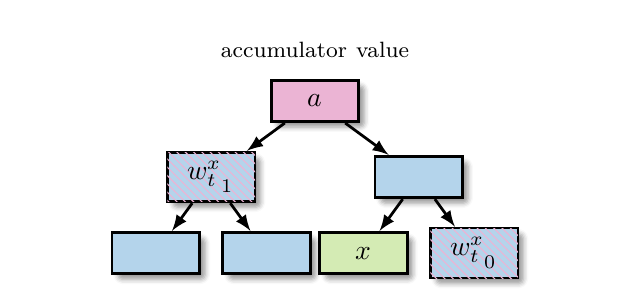
\begin{tikzpicture}[-latex,
every node/.style = {shape=rectangle, line width=1pt, color=black,
  draw, align=center, text width=2.5em, minimum height=1.5em,
  blur shadow={shadow blur extra rounding, shadow xshift=2pt, shadow yshift=-2pt},
  fill=boxbg},
witness/.style = {
  postaction = { pattern=north west lines }, pattern color=boxredish
},
note/.style = {
  fill=none, color=white, text width=20em, blur shadow={shadow opacity=0}, text=black
},
  edge from parent/.style = {line width=1pt, draw},
level 1/.style={sibling distance=7.5em},
level 2/.style={sibling distance=4em},
level 3/.style={sibling distance=3.5em},
level distance=2.75em
]
\node (root) [fill=boxredish] {$a$}
  child { node [witness] {${w^x_t}_1$}
    child { node {} }
    child { node {} }
  }
  child { node {}
    child { node [fill=boxlime] {$x$} }
    child { node [witness] {${w^x_t}_0$} }
  };

\node [above of=root, yshift=-1em, draw, note] {{\footnotesize accumulator value}};

\end{tikzpicture}

\end{center}

\begin{textblock*}{5cm}(3.3cm,6.7cm)
\begin{gather*}
\textrm{Merkle proof } \{ ({w^x_t}_0, right), ({w^x_t}_1, left) \} \\
a = h({w^x_t}_1 || h(x || {w^x_t}_0))
\end{gather*}
\end{textblock*}
\end{frame}

\begin{frame}{Merkle tree as an Accumulator}
\begin{center}
    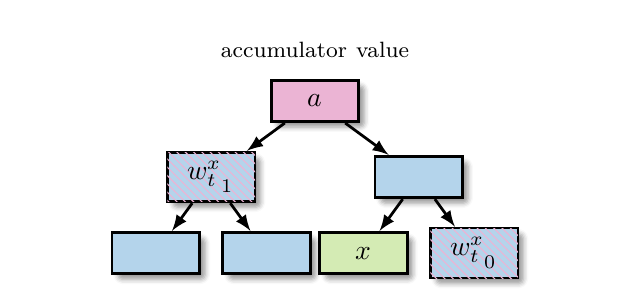
\begin{tikzpicture}[-latex,
every node/.style = {shape=rectangle, line width=1pt, color=black,
  draw, align=center, text width=2.5em, minimum height=1.5em,
  blur shadow={shadow blur extra rounding, shadow xshift=2pt, shadow yshift=-2pt},
  fill=boxbg},
witness/.style = {
  postaction = { pattern=north west lines }, pattern color=boxredish
},
note/.style = {
  fill=none, color=white, text width=20em, blur shadow={shadow opacity=0}, text=black
},
  edge from parent/.style = {line width=1pt, draw},
level 1/.style={sibling distance=7.5em},
level 2/.style={sibling distance=4em},
level 3/.style={sibling distance=3.5em},
level distance=2.75em
]
\node (root) [fill=boxredish] {$a$}
  child { node [witness] {${w^x_t}_1$}
    child { node {} }
    child { node {} }
  }
  child { node {}
    child { node [fill=boxlime] {$x$} }
    child { node [witness] {${w^x_t}_0$} }
  };

\node [above of=root, yshift=-1em, draw, note] {{\footnotesize accumulator value}};

\end{tikzpicture}

\end{center}

Each time you put a new item, accumulator value (Merkle root, $a$) and witness (Merkle proof, $w^x_t$)
should be updated.
\end{frame}

\begin{frame}{Accumulator Types}
  \begin{description}
    \item[dynamic accumulator] can remove members.
    \item[universal accumulator] can tell whether the item is \emph{not} in the set, too.
  \end{description}
\end{frame}

\begin{frame}{Let's Reduce the State Size!}
Ethereum uses Patricia Merkle trie accumulator now, and disregards non-state
information (such as receipts) because it is unreachable from transactions (smart contracts).

But witness can be prepared by off-chain computation.
Non-state information (history) can be useful in future.

If there are efficient accumulators for append-only data (history), we could
make a contract use history than state, and adapt dual accumulator VM.
History-driven Application could use very small state (actually one hash due to
TrueBit or zero knowledge) or state only for temporary purposes.
\end{frame}

\begin{frame}{Low update frequency accumulator\footnote{https://ethresear.ch/t/history-state-and-asynchronous-accumulators-in-the-stateless-model/287}}
It is called by many names: asynchronous accumulator\footnote{https://eprint.iacr.org/2015/718.pdf},
Merkle mountain range (MMR)\footnote{https://petertodd.org/2016/delayed-txo-commitments}, delayed (U)TXO commitment and so on.

Even if accumulator value and witness are not synchronous, i.e.,
witness is older than accumulator value or
accumulator value is older than witness,
it can verify a member. Then updates can be delayed.
It makes $log(n)$ times updates, and take up $log(n)$ times space (i.e., moutain summits).
\end{frame}

\begin{frame}{Step 1/4}
\include{dia3}
\end{frame}

\begin{frame}{Step 2/4}
    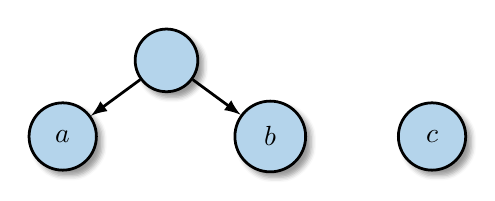
\begin{tikzpicture}[-latex,
every node/.style = {shape=circle, line width=1pt, color=black,
  draw, align=center, text width=1.5em, minimum height=1.5em,
  blur shadow={shadow blur extra rounding, shadow xshift=2pt, shadow yshift=-2pt},
  fill=boxbg},
witness/.style = {
  postaction = { pattern=north west lines }, pattern color=boxredish
},
note/.style = {
  fill=none, color=white, text width=20em, blur shadow={shadow opacity=0}, text=black
},
  edge from parent/.style = {line width=1pt, draw},
level 1/.style={sibling distance=7.5em},
level 2/.style={sibling distance=4em},
level 3/.style={sibling distance=3.5em},
level distance=2.75em
]
\node {}
  child { node {$a$} }
  child { node (b) {$b$} };
\node [right of=b,xshift=3em] {$c$};

\end{tikzpicture}

\end{frame}

\begin{frame}{Step 3/4}
    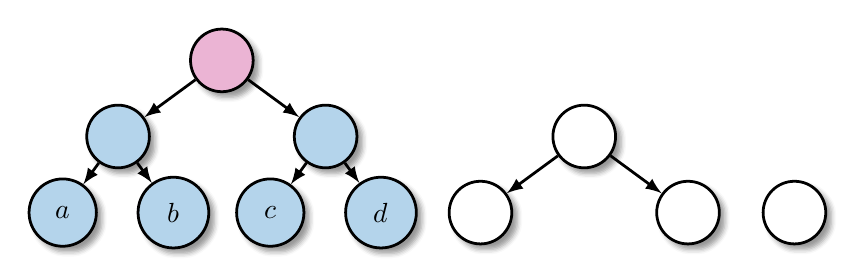
\begin{tikzpicture}[-latex,
every node/.style = {shape=circle, line width=1pt, color=black,
  draw, align=center, text width=1.5em, minimum height=1.5em,
  blur shadow={shadow blur extra rounding, shadow xshift=2pt, shadow yshift=-2pt},
  fill=boxbg},
witness/.style = {
  postaction = { pattern=north west lines }, pattern color=boxredish
},
note/.style = {
  fill=none, color=white, text width=20em, blur shadow={shadow opacity=0}, text=black
},
  edge from parent/.style = {line width=1pt, draw},
level 1/.style={sibling distance=7.5em},
level 2/.style={sibling distance=4em},
level 3/.style={sibling distance=3.5em},
level distance=2.75em
]
\node [fill=boxredish] {}
  child { node {}
    child { node {$a$} }
    child { node {$b$} }
  }
  child { node (r) {}
    child { node {$c$} }
    child { node (d) {$d$} }
  };
\node [right of=r,xshift=6.5em,fill=white] {}
  child { node [fill=white] {} }
  child { node [fill=white] (bottom) {} };
\node [right of=bottom,xshift=1em,fill=white] {};

\end{tikzpicture}

\end{frame}

\begin{frame}{Step 4/4}
\include{dia6}
\end{frame}

\begin{frame}{Double-Batched Merkle Log Accumulator}
  By stacking two MMRs, double-batched merkle log accumulator seems to be best candidate.\footnote{https://ethresear.ch/t/double-batched-merkle-log-accumulator/571}

  ...(diagram here)...
\end{frame}

\begin{frame}
  \begin{quote}
    if you then use a model where users delay sending receipts as long as possible and only use receipts to create new receipts then you’ve basically reinvented the UTXO model.
  \end{quote}
\end{frame}

\section{Let's Extend It Further}

\begin{frame}{Dynamic Accumulator for State}
  We can make a dynamic accumulator by using an append-open accumulator.\footnote{https://ethresear.ch/t/a-cryptoeconomic-accumulator-for-state-minimised-contracts/385}
  We use \texttt{[add, o]} and \texttt{[del, o]} records instead of the sole items.
  It looks like an event sourcing database.
  Conflict proofs may be prevented by economic incentives.
\end{frame}

\begin{frame}{State Minimised Execution\footnote{https://ethresear.ch/t/state-minimised-executions/748}}
  We can replace stateful shards with log shards\footnote{https://ethresear.ch/t/log-shards-and-emv-abstraction/747}.
  On-chain validators will be replaced with off-chain executors such as TrueBit.
  Stateful executos make virtual transactions without witness possible.
\end{frame}

\end{document}
